\chapter{Olhó-passarinho}\label{chap:chap4}

Neste capitulo será abordado a ferramenta desenvolvida com a descrição da arquitetura sistema implementado, do processamento da informação espaço-temporal e da sua integração com a informação visual de modo a aplicar a tarefa de \textit{clustering}. Por fim será apresentado a visualização dos resultados ilustrativos e consequentemente a sua discussão. 

\section{Arquitetura do sistema}

A arquitetura do sistema desenvolvido é apresentado na figura~\ref{fig:archsys}. Este apresenta uma divisão entre os serviços externos e o serviço interno que representa o modelo desenvolvido. Este modelo foi desenhado de modo a que existisse uma separação entre o tratamento de toda a parte de processamento dos dados e a visualização, existindo assim um \textit{back-end} com todos os ficheiros e módulos desenvolvidos e um \textit{front-end} que representa a aplicação web para visualização dos resultados. No \textit{back-end} existe também uma divisão entre dois módulos fundamentais, o módulo de processamento da informação visual, responsável por tratar a informação das imagens como descrito no Capítulo~\ref{chap:chap3}, de modo a que essa informação possa ser utilizada pelo módulo responsável pelo processo de \textit{Data Mining} já desenvolvido no TweeProfiles~\cite{Cunha2013}. 

\begin{figure}
\centering
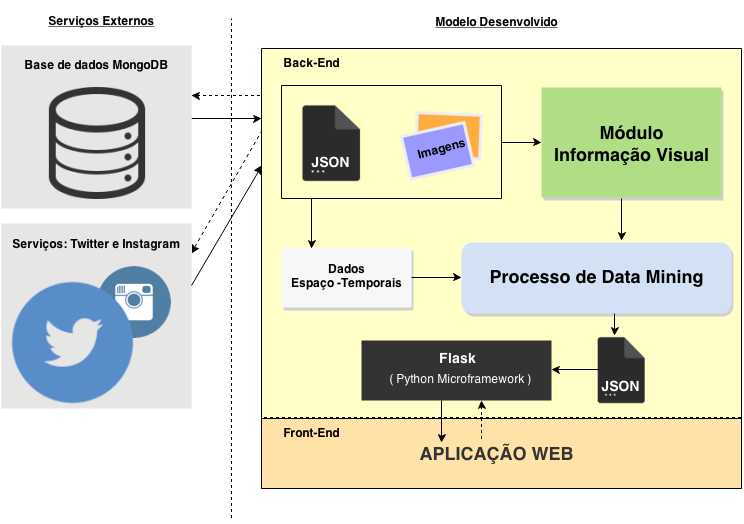
\includegraphics[width=1.0\linewidth]{./figures/arquitetura_sistema}
\caption{Arquitetura do sistema completo}
\label{fig:archsys}
\end{figure}



\section{Informação espaço temporal}



\section{Clustering da informação visual, espacial e temporal}

\section{Visualização}

\section{Resultados ilustrativos}